Hệ thống Diamond Stay được chia thành các module sau:
\begin{itemize}
	\item \textbf{Module 1 \textcolor{red}{(Tân)}:} Duyệt thông tin về yêu cầu thêm chỗ ở mới từ chủ nhà (Dành cho quản lí hệ thống) 
	\item \textbf{Module 2 \textcolor{red}{(Tân)}:} Quản lí khuyến mại (Khuyến mại của chủ nhà và khuyến mại của hệ thống).
	\item \textbf{Module 3 \textcolor{red}{(Tín)}:} Bình luận và rating cho nhà.
	\item \textbf{Module 4 \textcolor{red}{(Bảo)}:} Yêu cầu tạo tin mới, quản lý các tin đã gửi 
	\item \textbf{Module 5 \textcolor{red}{(Khoa)}:} Tìm kiếm và lọc kết quả; Đặt phòng homestay 
	\item \textbf{Module 6 \textcolor{red}{(Cường)}:} Theo dõi tình trạng đặt phòng cho chủ nhà
	\item \textbf{Module 7 \textcolor{red}{(Cường)}:} Các chức năng về nhắn tin cho khách thuê
	\item \textbf{Module 8 \textcolor{red}{(Cường)}:} Các chức năng về nhắn tin cho chủ nhà 
\end{itemize}
\newpage 
\begin{figure}[H]
	\centering
	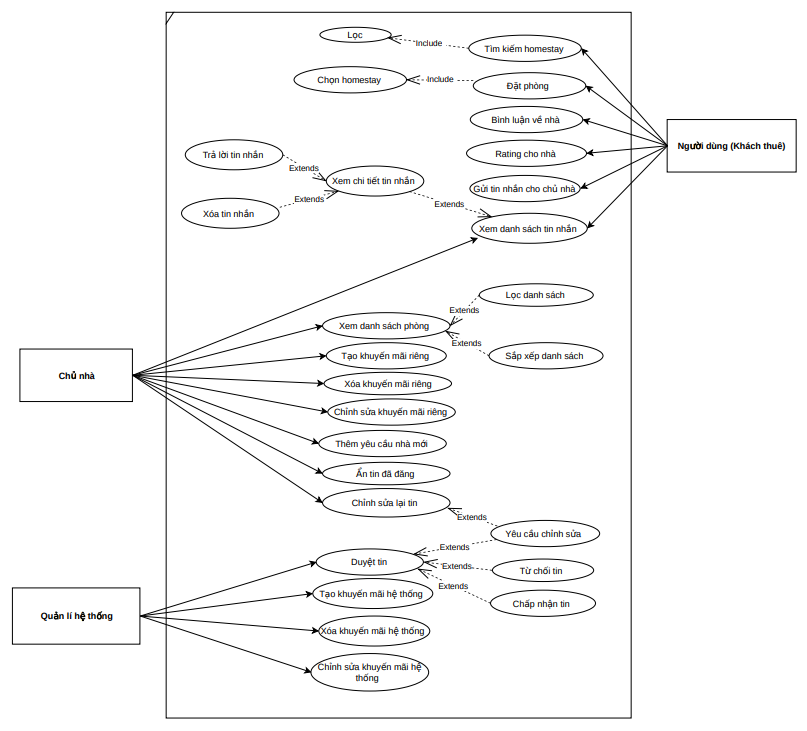
\includegraphics[width=17cm, height= 17cm]{Image/ucFull.png}
	\vspace{0.5cm}
	\caption{Lược đồ usecase của toàn hệ thống}
\end{figure}